\section{Discussion and Implications}\label{sec:discuss}
%
% goal: 1 page
%
% content is commented out and to be edited and un-commented once the "Evaluation Section" takes shape

While the previous section focuses on the collected data and comparisons between
the three architectures, this section summarizes the relevant points to consider
from our study, which should be taken into account when moving forward.

\subsection{Performance Metrics}
The de facto performance metric reported in HPC is \unit[]{flop/s}. Reporting \unit[]{flop/s} is not limited to applications that are compute-bound. Benchmarks that are designed to resemble realistic workloads, e.g., the
memory-bound HPCG benchmark, typically report performance in \unit[]{flop/s}. The proxy-/mini-apps in this study as well typically report \unit[]{flop/s} despite only six out of 20 proxy-/mini-apps we analyze in this study appearing to be
compute-bound (including NGSA that is bound by ALUs, not FPUs). We
argue that convening on reporting relevant metrics would shift the focus of the community to be less \unit[]{flop/s}-centered.
%It is important to mention that reporting only time-to-solution and scalability, without reporting performance, is a common pitfall that distorts the interpretation of results in HPC~\cite{hoefler_scientific_2015}.

\subsection{Considerations for HPC Utilization by Scientific Domain}\label{ssec:workload_util}
%
\begin{comment}
\begin{figure}[tbp]
    \centering
    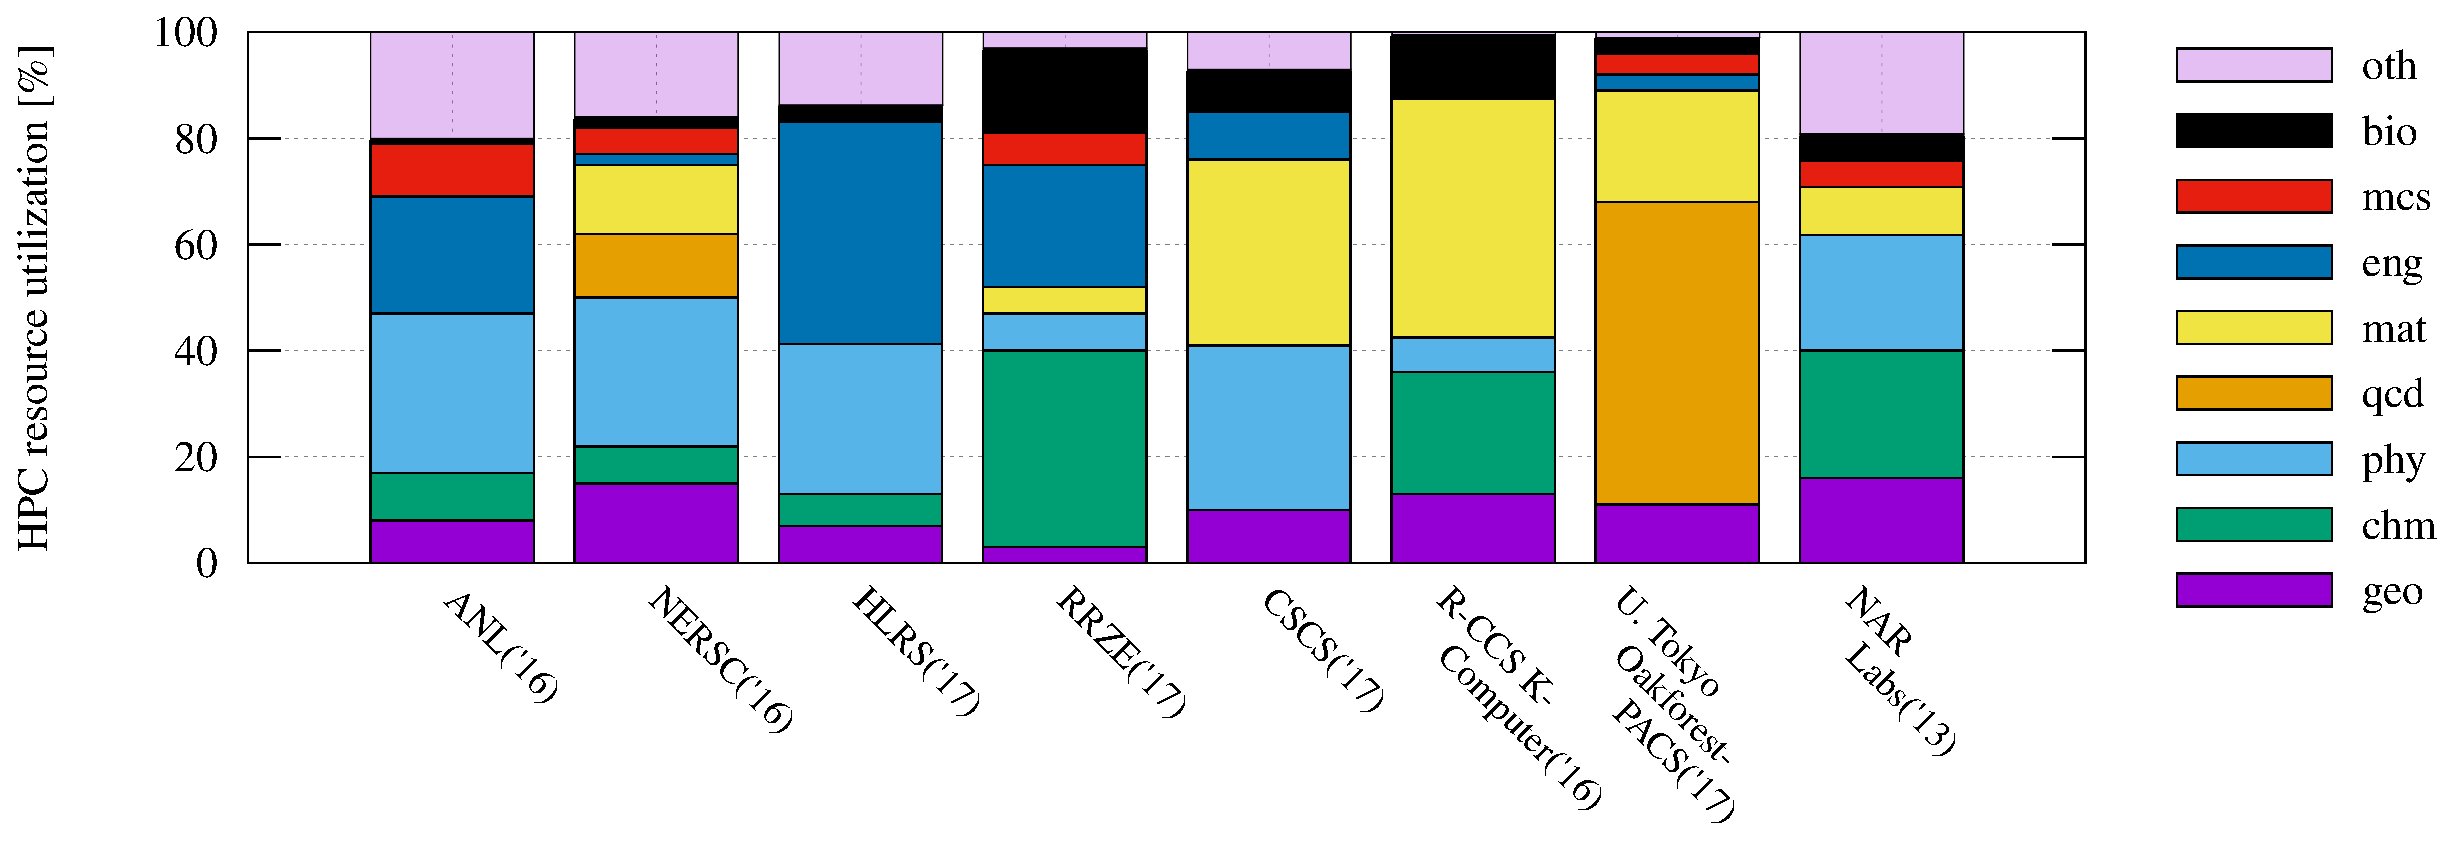
\includegraphics[width=\linewidth]{sys-util}
    \caption{\label{fid:disc:breakdown} Annual HPC site/system utilization by domain; Labels acc. to Table~\ref{table:APP}: \texttt{geo} = Geo-/Earthscience, \texttt{chm} = Chemistry, \texttt{phy} = Physics, \texttt{qcd} = Lattice QCD, \texttt{mat} = Material Science/Engineering, \texttt{eng} = Engineering (Mechanics, CFD), \texttt{mcs} = Math/Computer Science, \texttt{bio} = Bioscience, \texttt{oth} = \textit{Other}}
\end{figure}
\end{comment}
%
This paper highlights the diminishing relevance of \unit[]{flop/s} when
considering the actual requirements of representative proxy-apps.
The relevance of \unit[]{flop/s} on a given supercomputer can be further
diminished when considering the analysis of node-hours spent yearly on
different scientific domains at supercomputing facilities.
Figure~\ref{fid:disc:breakdown} summarizes the breakdown of node-hours by
scientific domain for different supercomputing facilities (based on yearly
reports of mentioned facilities). For instance, by simply mapping the scientific
domains in Figure~\ref{fid:disc:breakdown} to representative proxies,
ANL's ALCF and \mbox{R-CCS's} K-computer would be achieving $\approx$14\% and
$\approx$11\%, respectively, of the peak \unit[]{flop/s} when projecting
for the annual node-hours. %oversomplification?
It is worth mentioning that the relevance of \unit[]{flop/s} is even more
of an issue for supercomputers dedicated to specific workloads: the relevance of
\unit[]{flop/s} can vary widely. For instance, a supercomputer dedicated
mainly to weather forecasting, e.g., the~\unit[18]{Pflop/s} system recently
installed at Japan's Meteorological Agency~\cite{japan_meteorological_agency_jma_jma_2018},
should give minimal relevance to \unit[]{flop/s} since the proxy representing
this workload on that supercomputer achieves $\approx$6\% of the peak \unit[]{flop/s},
since those workloads are typically memory-bound. On the other hand, a
supercomputer dedicated to AI/ML such as ABCI, the world 5\textsuperscript{th}
fastest supercomputer as of June 2018, would put high emphasis on \unit[]{flop/s}
since deep learning workloads rely heavily on dense matrix multiplication operations.


\subsection{Memory-bound Applications}
As demonstrated in Figure~\ref{fig:flops}, the performance of memory-bound
applications is mostly not affected by the peak \unit[]{flop/s} available.
Accordingly, investment in data-centric architectures and programming models
should take priority over paying premium for \unit[]{flop/s}-centric systems.
In one motivating instance, during the investigation that NASA Ames Research
Center conducted to identify planned upgrade of the Pleiades supercomputer in
2016~\cite{saini_performance_2016}, the study concluded that the performance gain from upgrading to
Intel Haswell processors was insignificant in comparison to using the older
Ivy Bridge-based processors (the newer processor offered double the peak
\unit[]{flop/s} at almost the same memory bandwidth). And hence the choice was only do a partial upgrade to Haswell processors.

\subsection{Compute-bound Applications}
Investing more in data-centric architectures to accommodate memory-bound
applications can have a negative impact on the remaining minority of
applications: compute-bound applications. Considering the market trends that
are already pushing away from dedicating the majority of chip area to
FP64 units, it is likely that libraries with compute-bound code (e.g., BLAS)
would support mixed precision or emulation by lower precision FPUs. The
remaining applications that do not rely on external libraries might suffer a
performance hit.

%\subsection{More Diversity in FPUs\cJD{not less?}}
% - option: suggest to ditch fp32 and emulate fp32 ops in fp64 units
% - mixed precision can't work (requ. hand tuning in each app) -> not practical
% - compute bound codes -> what if no FP64 anymore in new chips -> what will they do?


% - themes: time-to-solution is most important metric
% - instructions doesn't matter too much because most are memory-bound
% - apps have different requirements
% - people need to dive deeper into their workloads
% - suggestion: decouple notion of hpc apps need high FP64 and which architecture to choose => see if NASA has papers on their design choices?!
% - breakdown of node-hours on science fields across many hpc centers


